
\documentclass{IOS-Book-Article}

\usepackage{mathptmx}
\usepackage{graphicx}
\usepackage{listings}
\usepackage{booktabs}
%\usepackage{times}
%\normalfont
%\usepackage[T1]{fontenc}
%\usepackage[mtplusscr,mtbold]{mathtime}
%
\def\hb{\hbox to 10.7 cm{}}

\begin{document}

\pagestyle{headings}
\def\thepage{}

\begin{frontmatter}              % The preamble begins here.


%\pretitle{Pretitle}
\title{Solving Sparse Linear Systems of Equations using Fortran Coarrays}

%\markboth{}{September 2016\hb}
%\subtitle{Subtitle}

\author[A]{\fnms{Ambra} \snm{Abdullahi Hassan}%
},
\author[A]{\fnms{Valeria} \snm{Cardellini}}
and
\author[B]{\fnms{Salvatore} \snm{Filippone}}

\address[A]{University of Rome Tor Vergata}
\address[B]{Cranfield University}

\begin{abstract}
Coarrays have been part of the Fortran standard since
Fortran 2008 and provide a syntactic extension of Fortran to
support parallel programming, often called Coarray Fortran (CAF). 
Although MPI is the de facto standard for parallel programs running on
distributed memory systems and little  scientific software is  written in
CAF, many scientific applications could benefit from the use of CAF.  
We present the migration from MPI to CAF of the libraries PSBLAS  and
MLD2P4 for the solution of large systems of equations using iterative
methods and preconditioners.  
In this paper we describe some investigations for implementing the
necessary communication steps in PSBLAS and MLD2P4 and provide
performance results obtained on linear systems arising from
discretization of 2D and 3D PDEs.    
\end{abstract}

\begin{keyword}
CAF, MPI, numerical linear algebra, sparse linear systems
\end{keyword}
\end{frontmatter}

%\markboth{September 2016\hb}{September 2016\hb}
%\thispagestyle{empty}
%\pagestyle{empty}


\section{Introduction}

Fortran has been the dominant language in High Performance
Computing and still is a very important player in the field. In past
couple of decades, the language has changed significantly,  and now 
supports class abstractions, object-oriented programming, pure
functions, and coarrays~\cite{Metcalf:2011:MFE}.  
Coarrays have been part of the Fortran standard since
Fortran 2008 and provide a syntactic extension of Fortran to
support parallel programming; in the sequel we will use Fortran
instead of CAF to highlight the fact that today the parallelization is
an integral part of the language.
Following the  Partitioned Global Address Space programming model,
in Fortran the program is replicated among a certain number of images,
executing asynchronously. 
The PGAS model combines elgance  and simplicity, by allowing one-sided
communications, and potentially reducing synchronization and code 
complexity. 
Coarrays are  a language-based approach, meaning that a quality
compiler implementation can consider both serial and communication
aspects in optimizing the generated code.
If the available  compiler also provides support for accelerator
programming, e.g. by implementing OpenAcc, the programmer can readily
get a dual benefit from the combined use of PGAS and accelerator
programming models. 


The Message Passing Interface (MPI) defines a suite of functions for
communication exchange between processes. MPI  is
library-based:  it is in principle independent from any specific
compiler, but the user  is bound to the vendor's fine-tuning of the
MPI library implementation~\cite{Garain:2015}.

At present  MPI is the de facto standard for parallel programs running
on distributed memory systems and few scientific softwares are written in
CAF; it is our belief that many scientific applications could
benefit from the use of the PGAS model implemented in coarrays; to
realize the potential, we have to analyze the impact of 
 Coarrays  on performance and quality of scientific software.

In this paper we focus on the solution of large and sparse linear
systems of equations and we propose the migration of the
PSBLAS~\cite{PSBLAS} and MLD2P4~\cite{mld-toms} libraries.

The first one implements various iterative solvers while the second
exploits most of the communications subroutines in PSBLAS to implement
multigrid preconditioners. Using the combinations of the two
libraries, we can compare performances of real-world problems in MPI
and in CAF.

Few attempts to implement multigrid solvers in CAF have been made, for
example in~\cite{Numrich:1998} (in which early versions of CAF and MPI
have been used).  In~\cite{Garain:2015} a comparison between MPI3 and
CAF is presented for spectral techniques, multigrid techniques and for
applications drawn from computational fluid dynamics. It shows that
Cray implementations of MPI3 and CAF performances in message passing
are comparable (with CAF slightly outperforms MPI3 in some cases), and
it points out the advantages of CAF when it comes to ease of
implementation. In this paper we compare performances of CAF and MPI
on problems arising from discretization of 2D and 3D PDEs, using
preconditioned iterative methods (also with multigrid
preconditioners). We used the GNU compiler and the OpenCoarray
library~\cite{PGAS14}, both opensource and easily accessible.

\section{Fortran Coarrays}

Coarrays extend the original Fortran language with minimal syntactic 
constructs, allowing for Single Program Multi Data (SPMD) parallel
programming.  
It follows the Partitioned Global Address Space (PGAS) parallel
programming model, which it is an effective alternative combining the
advantages of the SPMD programming style for distributed memory
systems with the data referencing semantics of shared memory systems.  
In the PGAS model, multiple ``images'' participate into  the global
address space, each one of them having a local portion and access to
the shared portion of the address space. 
Other  languages based on the PGAS model include Unified Parallel C
(UPC)~\cite{UPCSpec},  Chapel~\cite{chapel}, X10~\cite{Charles:2005}
and SHMEM.

With coarrays most of the parallel bookkeeping is handled behind the scene by
the compiler;  compared to MPI the parallelization is easier to
follow, the code is shorter and less complex. We can think, for
example, of the burden of transferring a non-contiguous portion of an
array using MPI, a task that is achieved with a single statement, 
or  that in  CAF there is no need to write explicit and separate code
for sending and receiving a message. 

Coarrays are supported by Cray, Intel and  GNU 
compilers; in the GNU compiler the code is translated by emitting
calls into an API  implemented by the open source openCoarrays
project, which in turn provides two different transport
layer implementations  based on MPI and on GASNet~\cite{PGAS14}.  

In the Fortran language the program is replicated a certain number of
times and each replica, called an image, executes asynchronously
with its own set of data objects.  
 Variables  declared as \emph{coarrays} become visible to all images,
 thereby implementing a locally shared portion of the address space;
 the syntax uses \emph{coindices} indicated by square brackets, with
 an appearance very similar to normal array syntax:
{\small
\begin{lstlisting}
integer ::co_a[*],co_b(n,m)[*]
\end{lstlisting}}
Any statement with coindices indicates access of the variable on a
(possibly) remote image, thus enabling data exchange:
{\small
\begin{lstlisting}
co_a[1]=co_a
\end{lstlisting}}
Dropping a coindex implicitly refers to the local version of the
variable. 
Each image is assigned a unique index, through which the programmer
can control the flow of the execution. Image indices start from 1 and
can be retrieved using the intrinsic function $this\_image()$;  the
total number of images can be retrieved using the function
$num\_images()$. %% The total number of images can be 
%% different from the total number of processors and it can be decided at
%% compile, link or runtime depending on the implementation.
The exact mechanism to determine how many images will be executed
depends on the compiler's implementation: most implementation use a
runtime scheme similar to (or directly based on) that of MPI. 

Data transfers in Fortran are asynchronous and non-blocking;
to prevent  deadlock and race conditions, the programmer has to ensure
consistency through the use of synchronization statements.

The \verb|SYNC ALL| statement corresponds to a global barrier (all
images waiting for each other) while \verb|SYNC IMAGES| allows for
 synchronization restricted within a subset of images.

In the Fortran 2015 language a number of extensions to the original
coarray language have been introduced; among them are the
\verb|EVENTS|, which implement an asynchronous notification
mechanism. 
An image can use an \verb|EVENT POST| statement to notify another
image without having to go through a full two-way handshaking; in
particular, there is no tie to the 
execution of a matching \verb|EVENT WAIT| by the receiving image .
This facility allows for \emph{one-sided} synchronization
strategies.   

Besides  explicit synchronizations, in a Fortran program there can be
implicit synchronization points the programmer must be aware of, 
because they can obviously have a significant impact on  performance. 
An example of an implicit synchronization point is allocation or
deallocation of a coarray: 
{\small
\begin{lstlisting}
integer, allocatable :: co_a(:,:)[:]
allocate(co_a(i,10)[*])
\end{lstlisting}}
Code executed between any two synchronizatoin points can be optimized
by the  compiler using all common techniques and heuristics  as if
it was a purely serial code~\cite{CAF}. 

\section{PSBLAS and MLD2P4}

Many  scientific and engineering applications require solving a
large sparse linear system of equations efficiently on parallel
machines;  in these cases direct solvers such as Gaussian elimination
are often ineffective and iterative solvers are a common alternative.

These techniques produce a sequence of approximate solutions, ideally
converging to the real one. Rate of convergence of iterative methods
depends upon the condition number of the matrix, hence iterative
methods usually involve a transforation of the original matrix into a
more well-conditioned one. This transformation is called a
preconditioner~\cite{barrett1994templates}. Krylov methods today the
most commonly used iterative techniques; they are based on minimizing
the residual $r=b-Ax$ over a certain linear or affine 
subspace~\cite{ipsen1998idea}. The Conjugate Gradient 
(CG)~\cite{shewchuk1994introduction}, the Generalized Minimal Residual  
(GMRES)~\cite{saad1986gmres} and the Biconjugate Gradient
(BiCG)~\cite{van1992bi} are popular Krylov method variants.

Multigrid methods have also shown promising results in solving linear
systems arising from partial differential equations and they have the
nice property that they can achieve convergence rates which are, in
theory, independent of the mesh size~\cite{saad2003iterative}. 
Multigrid can be used as stand-alone solvers~\cite{brandt1977multi}
or as preconditioner for a Kylov subspace
method~\cite{bramble1990parallel}.  
PSBLAS is a library of Basic Linear Algebra Subroutineas for parallel
sparse applications is designed to handle parallel implementation of
iterative solvers for sparse linear systems. It is implemented if
object-oriented Fortran 2003; the serial computations are based on an
implementation of the serial sparse BLAS originally defined
in~\cite{duff2002overview}, while the inter-process 
massage exchanges are encapsulated in an application layer based by
default on MPI. The PSBLAS library contains, among 
others, 
subroutines for sparse-matrix-by-dense-matrix multiplication, sparse
triangular system solution, dot product, sparse matrix and data
distribution preprocessing. 
While addressing a distributed memory execution model the current
PSBLAS design does not preclude different implementation pradigms. 
MLD2P4 (Multi-level Domain Decomposition Parallel Preconditioners
Package based on PSBLAS) is a package for parallel algebraic
multilevel preconditioners. A purely algebraic approach is used and no
information about the underlying physical grid is needed to build the
preconditioner. MLD2P4 preconditioner are intended to be used in
conjuction with the iterative solvers available in the context of
PSBLAS.

Since in MLD2P4 inter-process data communiations is managed through
PSBLAS, writing a CAF version give us dual benefit: first, we can compare MPI and CAF on Krylov subspace methods and simple preconditioners, using PSBLAS; secondly, we can compare MPI and CAF on multilevel preconditioners, since MLD2P4 data communication is actually managed on PSBLAS. 
Additionally, since both PSBLAS and MLD2P4 are open source, once the
CAF version is released CAF programmers will be able to use them
inside their scientific application. 

 
\section{Iterative solver Implementation}
We converted the PSBLAS code gradually from MPI to CAF, thus having
the two communication strategies coexisting in the same code.  
We detected three communication patterns to modify:
\begin{enumerate}
\item The halo exchange
\item Collective subroutines
\item Point-to-point communication in data distribution
\end{enumerate}
In the following, we address the three patterns  separately.

\subsection{Halo Exchange}

The data distribution in  PSBLAS~\cite{PSBLAS} is best described by
referring to an underlying physical problem, such as a PDE discretized
on a mesh.
Each point in the discretization mesh corresponds to a variable and,
consequently, to an index in the coefficient matrix column space;
moreover, for each mesh point there is an equation, corresponding to a
matrix row. We say that index $i$ depends upon index $j$ whenever $a_{ij}\neq0$.  
In the process of distributing data among processes, the original
domain is divided into subdomains, with points (and the corresponding
equations) in the subdomain assigned to a process.  In each subdomain
a boundary point is a point depending on points from different
domains, which are called halo points. 
When performing e.g. a matrix-vector product, the
values corresponding to halo points will be requested from other
processes, with and the amount of exchanged data given by the number 
of boundary points.   This is a so-called halo exchange 
operation; we can think of halo exchange as a sparse all-to-all
communication (\verb|MPI_ALLTOALLV|). It is sparse in the  sense that
in a good data distribution, each subdomain only interacts with a
small subset of all other subdomains. 
\begin{figure}
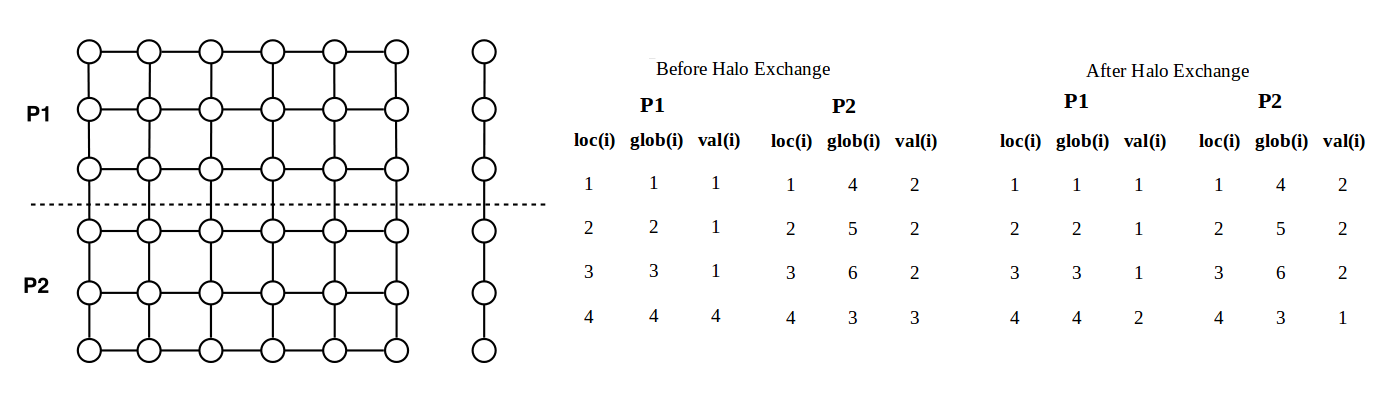
\includegraphics[height=1.5in, width=4.65in]{halo2.png}
\caption{Example of halo exchange on 2 images. }
%\label{classes}
\end{figure}
In  PSBLAS the halo exchange is by default reimplemented in terms of
point-to-point operations; this is because the basic 
\verb|ALLTOALLV| operation is not commonly optimized for sparse
interactions.


The subroutine performing the exchange takes a list of dependencies as
input, consisting  of variable size blocks, one for each of the
communication to perform. Each  block contains the remote process with
which to  exchange data, the number and indices of elements to send,
and the number and indices of elements to receive.
%% The ordering of the blocks, determines the sequence in which communications
%% take place, is defined through an internal algorithm. 
For the MPI version we can choose between different implementations; 
the halo\_exchange can thus happen through a single call to
MPI\_ALLTOALLV, by using send and receives communications in
synchronized pairs, or it can be split between 
two separate \emph{send} and \emph{receive} calls. In the latter case
the programmer needs to ensure that for each \emph{send} invocation
there is a matching \emph{receive}; this is very general, but requires
some sort of explicit or implicit buffering of the send data. 
If the two steps are concatenated in the same call, it is possible to
use minimal memory buffer space and maximize performance by employing 
\verb|mpi_irecv| calls.
The exchange then has the following logic flow: 
\begin{enumerate}
  \item Post non-blocking receives;
  \item Pack data into buffers and send; 
  \item Wait for the receive operations to complete; 
  \item Unpack data from the receive buffers. 
\end{enumerate} 
For structured grids partitioned along coordinate planes, the halo
exchange could be implemented with simple remote coarray accesses. The
situation is much more complicated if, as in PSBLAS, we want to handle
unstructured meshes and arbitrary domain partitionings. In this  case
the only way to proceed is to have matched lists of entries to be
retrieved and/or sent; a direct access of the remote entries could be
implementeed with indirect addressing, with a statement like
\lstset{language=Fortran} 
{\small
\begin{lstlisting}
x(rcv_idxs(1:nrcv(img))) =  x(rcv_idxs(1:nrcv(img)))[img]
\end{lstlisting}}
This is perfectly legal, but the implication is that the accesses on
the remote image require the indices to travel, and the resulting
efficiency would be dubious. The first approach we took then was to 
have a more ``cooperative'' handling of data packing between the
various processes, with the buffers declared as coarrays. 

When rewriting the halo exchange subroutine in CAF, we need to choose
if we want to perform the exchange operation using GET or PUT
operations.  
Let's assume that we need to pass a scalar value, stored on the
variable $a$ from image $1$ to image $2$. Since communications in CAF
are one-sided, this can be done in two ways: 
\lstset{language=Fortran} 
{\small
\begin{lstlisting}
if (this_image()==1) a[2] = a
\end{lstlisting}}
or
{\small
\begin{lstlisting}
if (this_image()==2) a = a[1]
\end{lstlisting}}
In the first case image $1$ performs a PUT operation; in the second
case, image $2$ performs a GET operation. We have implemented both
cases in PSBLAS, but preliminary tests  show that the PUT version
generally leads to a slightly smaller execution time.
Both versions require a coarray buffer. In the GET version it is
possible to incorporate the data exchange in the operation of packing
the sending data: in this case no other buffer is needed. For the PUT
version, it is still necessary to provide a separate receive buffer.

A key factor is the management of  allocation of coarrays in the
code. Since in CAF allocate and deallocate statements are implicit
synchronization barriers, they are significantly more expensive than
normal allocations, and therefore  they should be
avoided as much as possible.  Thus we declare communication
buffers with the \verb|save| attribute to enable reuse, and we only
need to reallocate occasionally when the size of the requested
exchange does not fit into the available space. 
%% \lstset{language=Fortran} 
%% \begin{lstlisting}
%%   if (psb_size(buffer) < xchg%max_buffer_size) then
%%     if (allocated(buffer)) deallocate(buffer)
%%     allocate(buffer(xchg%max_buffer_size)[*],stat=info)
%%     if (allocated(sndbuf)) deallocate(sndbuf)
%%     if (info == 0) allocate(sndbuf(xchg%max_buffer_size),stat=info)
%%     if (info /= 0) then
%%       info = psb_err_internal_error_
%%       call psb_errpush(info,name,a_err='Coarray buffer allocation')
%%       goto 9999
%%     end if
%%   end if
%% \end{lstlisting}
 With MPI the buffers are local, and since in most systems allocation
 is cheap we normally release the buffers to save memor.
Before showing performance results for  the halo exchange, we 
make a comparison between MPI and CAF for the halo exchange in terms
of impact on software quality.  
The interface for the halo exchange in psblas is \verb|psi_swapdata|;
this interface requires different implementations for the various data
types  in PSBLAS (integer, real and complex), and  for both single
vectors and multivectors, i.e. sets of related vectors stored as
``tall and skinny'' 2D matrices. Any benefits from code simplification
are thus accrued multiple times.

Comparing the  MPI and the CAF versions we see that there are benefits
in : 
\begin{enumerate}
\item Number of input variables: the MPI version requires 12 input
  variables, while the CAF version requires 8 input variables 
\item Number of lines of code for the single implementation is 185 for
  MPI and 116 for CAF;  
\end{enumerate}
Note that many of the lines of code are actually devoted to  tests for error
conditions and other general tasks,  in common among the two versions;
the impact on the strict communication part of the code is even larger
than appears at first glance. 
  
\subsection{Collective Subroutines and Point-to-point in Data Distribution}

Here we take into account all the subroutines performing collective
communications, in which all images take part in the
communication. While rewriting the halo exchange using CAF leads to a
reduction in the number of lines in the code, in this case we can
expect an increasing in the length of the code. This is because MPI
provides an interface for most of the collectives we may need in
solving a sparse linear system in parallel.
The current language standard defines the following collectives: co\_broadcast, co\_max, co\_min, co\_sum, co\_reduce
Some of the collectives provided by MPI  we have investigated
reimplementing ourselves; in what follows we are typically emphasizing
simplicity over efficiency, a proper study of further implementation
techniques will be the subject of future work. In particular 
we have the implementations for the interfaces caf\_scatterv,
caf\_gatherv, caf\_allgatherv, caf\_allgatherv caf\_gather,
caf\_alltoallv and caf\_alltoall.  
As an example, the code implementing the caf\_alltoall looks like:
\lstset{language=Fortran} 
\iffalse
{\small
\begin{lstlisting}
  subroutine caf_alltoall(snd,rcv, m, info)
    implicit none
    integer(psb_ipk_), intent(in) :: m
    integer(psb_ipk_), intent(in) :: snd(:)
    integer(psb_ipk_), intent(out):: rcv(:), info
    !Local
    integer(psb_ipk_) :: me, np,i, snd_start, snd_finish, snd_tot
    integer(psb_ipk_), allocatable :: buffer(:)[:], rcv_start, rcv_finish
    if ( m < 0) then
      print*,'Error, m must be greater or equal to zero'
      info = -1
    endif
    me = this_image()
    np = num_images()
    snd_tot=m*np
    if (allocated(buffer)) deallocate(buffer)
    allocate(buffer(snd_tot)[*], STAT = info)
    if (info /= 0) then
       print*,'allocation error', info
       return
    endif
    rcv_start = (me-1)*m +1
    rcv_finish = rcv_start + m - 1
    do i=1,np
      snd_start = (i-1)*m +1 
      snd_finish = snd_start + m - 1
      if (rcv_finish > snd_tot) then
        print*,'Error, rcv_finish > snd_tot'
        info = -2 
	return
      endif
      if (snd_finish > size(snd,1)) then
        print*,'Error, snd_finish > size(snd,1)'
        info = -3 
      endif
      buffer(rcv_start:rcv_finish)[i]=snd(snd_start:snd_finish)
    enddo
    !sync to ensure all image has finishe the PUTs 
    sync all
    rcv(1:snd_tot)=buffer(1:snd_tot)
    if (allocated(buffer)) deallocate(buffer)
  end subroutine caf_alltoall
\end{lstlisting}}
\else
{\small
\begin{lstlisting}
    me = this_image()
    np = num_images()
    snd_tot=m*np
    rcv_start = (me-1)*m +1
    rcv_finish = rcv_start + m - 1
    do i=1,np
      snd_start = (i-1)*m +1 
      snd_finish = snd_start + m - 1
      buffer(rcv_start:rcv_finish)[i]=snd(snd_start:snd_finish)
    enddo
    !sync to ensure all image has finishe the PUTs 
    sync all
    rcv(1:snd_tot)=buffer(1:snd_tot)
\end{lstlisting}}
\fi
The actual code would contain a number of error checking options that
are not shown here for clarity.
For what it concerns the reduction operations, the \verb|co_reduce| is
already part of the standard, and here the difference in code is
obvious. For the  MPI version we have:
\begin{center}
{\small
\begin{lstlisting}
call psb_realloc(size(dat),dat_,iinfo)
dat_ = dat
if (iinfo == psb_success_) &
    & call mpi_allreduce(dat_,dat,size(dat),psb_mpi_r_dpk_,&
    & mpi_dnrm2_op,ictxt,info)

\end{lstlisting}}
\end{center}
whereas for  the CAF version we have a single statement: 
\begin{center}
{\small
\begin{lstlisting}
call co_reduce(co_dat_,caf_dnrm2)
\end{lstlisting}}
\end{center}
The CAF syntax is more compact and does not differentiate between
input and output variables, which suits perfectly our usage and
eliminates the need for  the extra euxiliary variable dat\_. 

%% Finally, we modified the psb\_matdist subroutines, an utility
%% subroutine that uses point-to-point communications to distribute a
%% matrix among processors according user defined data distribution. In
%% this case, for both MPI and CAF we are using one-sided
%% communications. In the case of CAF, to ensure performance
%% optimizations, we used events to ensure synchronization among
%% images.


\section{Results}
CAF and MPI versions of PSBLAS and MLD2P4 have been tested on matrices
generated by 2D and 3D PDEs. 
The experiments were carried out on the Yoda linux cluster, operated
by the Naples Branch of the CNR Institute for High-Performace
Computing and Networking. Its compute nodes consist of 2 Intel Sandy
Bridge E5-2670 8-core processors and 192 GB of RAM, connected via
Infiniband. 
Both PSBLAS, MLD2P4 and OpenCoarrays-1.9 have been compiled on the top
of MPICH-3.2 and GNU 7.1. 

In PSBLAS and MLD2P4 it is possible to create the matrix corresponding to the PDE $
-a_1\frac{\mathrm d}{\mathrm d x \mathrm d x} \left(u \right) -a_2\frac{\mathrm d}{\mathrm d y \mathrm d y} \left(u \right) +b_1\frac{\mathrm d}{\mathrm d x} \left(u \right) +b_2\frac{\mathrm d}{\mathrm d y} \left(u \right) +cu = f
$ for the 2D problem and $
-a_1\frac{\mathrm d}{\mathrm d x \mathrm d x} \left(u \right) -a_2\frac{\mathrm d}{\mathrm d y \mathrm d y} \left(u \right) -a_3\frac{\mathrm d}{\mathrm d z \mathrm d z} \left(u \right) +b_1\frac{\mathrm d}{\mathrm d x} \left(u \right) +b_2\frac{\mathrm d}{\mathrm d y} \left(u \right) b_3\frac{\mathrm d}{\mathrm d z} \left(u \right)
 + cu = f$ for the 3D problem. The user can set the parameter $idim$. The dimension of the grid is then $idim^2$ for the 2D case and $idim^3$ for the 3D case.
 The resulting linear system is solved using a Biconjugated Conjugate Gradient Stabilized (BiCGSTAB) with a Block Jacobi preconditioner. The iterations are stopped when the 2-norm of the residuals vector achieved a reduction by a factor of $10^{-9}$
 
First we tested weak scalability for a 2D problem by keeping (roughly) constant the number of lines per process (Table \ref{weak}). 


\begin{table}[]
\centering
\caption{Weak scalability test for a 2D problem ($a_1=a_2=\frac{1}{80}$, $b_1=b_2= \frac{1}{\sqrt{2}}$,  $c=0$ dim = $idim^2$)}
\label{weak}
\begin{tabular}{@{}rrrrr@{}}
\toprule
\multicolumn{1}{c}{np} & \multicolumn{1}{c}{idim} & \multicolumn{1}{c}{MPI} & \multicolumn{1}{c}{\begin{tabular}[c]{@{}c@{}}CAF \\ ($sync images$)\end{tabular}} & \multicolumn{1}{c}{\begin{tabular}[c]{@{}c@{}}CAF\\ (events)\end{tabular}} \\ \midrule
1                      & 250                      & 0.64                 & 0.90                                                                          & 0.89                                                                    \\
2                      & 350                      & 0.99                 & 1.03                                                                           & 1.0                                                                      \\
4                      & 500                      & 1.37                  & 1.58                                                                           & 1.33                                                                     \\
8                      & 700                      & 2.00                  & 2.20                                                                           & 3.88                                                                     \\
16                     & 1000                     & 3.03                  & 3.82                                                                           & 4.41                                                                     \\
32                     & 1400                     & 5.07                  & 5.36                                                                           & 6.10                                                                     \\
64              

      & 2000                     & 6.52                  & 6.81                                                                           & 7.79                                                                     \\ \bottomrule
\end{tabular}
\end{table}

For CAF, two versions of the halo exchange have been tested: one performing synchronization through the use of events, the other through the use of the $sync images$ statement. While we expected synchronization through events to perform better, we actually observed that the version with $sync images$ is faster especially on many processes. In this case, MPI and CAF versions have total execution times that are very similar. 
Secondly, strong scalability tests have been performed for both 2D and 3D problems. Again, halo exchange with sync images performs better: for this reason in the following we show only results for this case. Table \ref{strong} shows results for the 3D problem.
 
\begin{table}[]
\centering
\caption{Strong scaling for a 3D problem: BiCGSTAB with BJAC preconditioner ($a_1=a_2=a_3=\frac{1}{80}$, $b_1=b_2=b_3=\frac{1}{\sqrt{3}}$, $c=0$,$idim=200$}
\label{strong}
\begin{tabular}{@{}rrr@{}}
\toprule
\multicolumn{1}{c}{np} & \multicolumn{1}{c}{MPI} & \multicolumn{1}{c}{CAF} \\ \midrule
1                      & 88.7                  & 106                  \\
2                      & 46.3                  & 46.5                  \\
4                      & 34.9                  & 23.3                  \\
8                      & 1.72                  & 1.45                  \\
16                     & 7.31                  & 9.94                  \\
32                     & 5.71                  & 5.12                  \\
64                     & 4.04                  & 3.61                  \\ \bottomrule
\end{tabular}
\end{table} 

Finally, we show results for the 3D problem, using the multilevel preconditioner implemented in MLD2P4. BiCGSTAB is used, with a multiplicative multilevel preconditioner, smoothed decoupled aggregation algorithm. The iterations are stopped when the 2-norm of the residuals vector achieved a reduction by a factor of $10^{-6}$ and a Jacobi smoother is used. The coarsest level matrix is distributed among processes and an incomplete LU factorization is used to solve the coarsest level matrix. Results are shown in Table \ref{Strong2}. Again performances of MPI and CAF are comparable in term of execution time. In the table, both the preconditioner building time (tprec) and the solution time are shown (tsolve). 

\begin{table}[]
\centering
\caption{Strong scaling for a 3D problem: BiCGSTAB with with a 2 level preconditioner ($a_1=a_2=a_3=1$, $b_1=b_2=b_3=0$, $c=0$,$idim=200$}
\label{Strong2}
\begin{tabular}{@{}rrrll@{}}
\multicolumn{1}{l}{}   & \multicolumn{2}{c}{MPI}                                & \multicolumn{2}{c}{CAF} \\ \midrule
\multicolumn{1}{c}{np} & \multicolumn{1}{c}{tprec} & \multicolumn{1}{c}{tsolve} & tprec      & tsolve     \\ \midrule
1                      & 37.5                      & 35.8                       & 37.4       & 35.6       \\
2                      & 19.9                      & 27.1                       & 19.8       & 26.9       \\
4                      & 10.3                      & 15.5                       & 10.5       & 15.3       \\
8                      & 5.56                      & 8.46                       & 5.37       & 9.87       \\
16                     & 3.71                      & 5.64                       & 2.35       & 5.87       \\
32                     & 2.19                      & 3.68                       & 2.44       & 3.72       \\
64                     & 1.45                      & 4.0                        & 2.12       & 3.72       \\ \bottomrule
\end{tabular}
\end{table} 
  
\section{Conclusions}

We successfully obtained a first migration of the  PSBLAS library from
MPI to CAF. Since MLD2P4 
communication is based on the PSBLAS framework, most of MLD2P4
preconditioners can exploit underlying CAF communication with little
effort. We point out that in the migration from MPI to CAF we retained
as much as the original code and structure that we could. While this
can lead to CAF code which is not as clear and readable as it would be
if the original software was thought and written in CAF from the
beginning, we think that the previous examples show the capability of
CAF to express parallelism in a simpler way than MPI. In all cases,
CAF code is shorter, clearer and easier to read. However, the CAF
programmer need to provide an interface for most of MPI collective
subroutines, which can increase the lenght of the code.  

We tested both the MPI and CAF versions on problems arising from
discretization of 2D and 3D PDEs. Neither CAF nor MPI version has
shown a clear superiority in terms of performance, with execution time
almost identical in the two cases.  The initial migration from MPI to CAF
was achieved without  a loss of performance; however this is only the
first step. In future work we plan to explore in further detail possible
alternative strategies for critical operations, such as  remote
indirect addressing, usage of \emph{get} versus \emph{put} strategis
for one sided communications, and a thorough study of the \verb|EVENT|
facility performance. 

\section{Acknowledgments} 
This work has been partially funded  from the European Union's Horizon 2020 Research
and Innovation Programme under Grant Agreement No.~676629
(Project EoCoE).
% (call H2020-EINFRA-2015-1, project ID: 676629, \url{http://www.eocoe.eu}).
The authors wish to thank Dr. Pasqua D'Ambra (CNR, Napoli, Italy),
for her help in running the experimental tests.
 
\bibliographystyle{unsrt}
\bibliography{psblas-caf}

\end{document}
 
\begin{thebibliography}{99}
\bibitem{r6}
Numrich, Robert W., and John Reid. "Co-Array Fortran for parallel programming." ACM Sigplan Fortran Forum. Vol. 17. No. 2. ACM, 1998.
\bibitem{r7}
Metcalf, Michael, John Reid, and Malcolm Cohen. Modern Fortran Explained. Oxford University Press, 2011.
\bibitem{r8}
UPC Consortium. UPC Language Specifications, v1.2.
Tech Report LBNL-59208, Lawrence Berkeley
National Lab, 2005.
\bibitem{r10}
V. Saraswat, B. Bloom, I. Peshansky, O. Tardieu, and
D. Grove. The X10 language specification, v2.2.3,
2012.
\end{thebibliography}

